\documentclass[11pt]{article}

\usepackage{amsmath}
\usepackage{amssymb}
\usepackage{amsthm}
\usepackage{physics}
\usepackage[margin=1in]{geometry}
\usepackage{enumitem}
\usepackage{tikz}
\usetikzlibrary{arrows.meta,backgrounds}

\newcommand{\TpM}{T_p\mathcal M}
\newcommand{\TpsM}{T_p^*\mathcal M}
\newcommand{\TprsM}{T_p^{(r,s)}\mathcal M}
\newcommand{\Cinf}{C^\infty(\mathcal M)}
\newcommand{\prim}[1]{\mathrm{prim}_{#1}}

\title{Chapter 3 --- Topological Manifolds\\ \large Exercises}
\author{From Differential Geometry to General Relativity --- Study Companion}
\date{}

\begin{document}
\maketitle

\noindent This file is self-contained: everything needed to state and solve
the problems below is introduced inline, in the book's own notation, no
outside reference is required. Problems are organized by topic, following
the logical order in which the chapter builds up the theory; within each
topic, an introduction comes first (motivation, notation and definitions with
worked examples, common pitfalls), then problems (easy $\to$ hard), then
their solutions.

% =============================================================================
\section{Topological Spaces and Open Sets}
% =============================================================================

\subsection*{Motivation}

\paragraph{Why topology at all.}
Physics constantly uses the word ``nearby'': a limit, a trajectory without jumps, a field that varies smoothly, a small perturbation. In ordinary calculus on $\mathbb R^d$, ``nearby'' means ``at small distance''. In General Relativity, however, the distance itself is what the theory determines (the metric is the unknown of Einstein's equations), so before solving anything we must already be able to say which events are close to which, and which maps do not tear spacetime apart, using no metric at all. A \emph{topology} is the minimal structure that does this: it is just a chosen family of subsets, called \emph{open}, from which ``nearby'', ``limit'' and ``continuous'' can all be recovered. No distance, no coordinates and no calculus are needed.

\paragraph{What ``open'' is trying to capture.}
Think of an open set as a region that contains none of its own boundary: every point of it has some room around it that still lies inside the set (the inside of a disc, without its rim). Which properties should any family of such regions have? The empty region and the whole space qualify; two regions with room overlap in a region with room; gluing together any number of regions with room, however many, gives a region with room. The three axioms below are exactly these requirements, stated without any reference to distance.

\paragraph{The question the axioms answer.}
Does a set come with its topology, or is the topology an extra choice? Can the same set carry several different families of open sets that all satisfy the axioms? And is there always at least one family available, whatever the set? The finite example below shows that the same set can carry several topologies, and Problem~\ref{prob:discrete-indiscrete} settles the last question.

\subsection*{Notation and Definitions}

\subsubsection*{Powerset and topology}
Let $\mathcal M$ be a set. Its \emph{powerset} $\mathcal P(\mathcal M)$ is the set of all subsets of $\mathcal M$. A subset $\mathcal O\subseteq\mathcal P(\mathcal M)$ is a \emph{topology} on $\mathcal M$, written $\mathcal O_{\mathcal M}$, if:
\begin{enumerate}[label=(\arabic*)]
  \item $\emptyset\in\mathcal O_{\mathcal M}$ and $\mathcal M\in\mathcal O_{\mathcal M}$;
  \item for all $\mathcal U,\mathcal V\in\mathcal O_{\mathcal M}$, the intersection $\mathcal U\cap\mathcal V$ lies in $\mathcal O_{\mathcal M}$;
  \item for every index set $A$ and every family $\{\mathcal U_\alpha\}_{\alpha\in A}$ of elements of $\mathcal O_{\mathcal M}$ (indexed by $\alpha\in A$), the union $\bigcup_{\alpha\in A}\mathcal U_\alpha$ lies in $\mathcal O_{\mathcal M}$.
\end{enumerate}
Here an \emph{index set} $A$ is any set of labels used to name the members of a family: $\{\mathcal U_\alpha\}_{\alpha\in A}$ means ``one open set $\mathcal U_\alpha$ for each label $\alpha\in A$''. The set $A$ may be finite (e.g.\ $A=\{1,2,3\}$), countably infinite (e.g.\ $A=\mathbb N$) or uncountable (e.g.\ $A=\mathbb R$). The union of the family is
\[
\bigcup_{\alpha\in A}\mathcal U_\alpha:=\{p\in\mathcal M\mid p\in\mathcal U_\alpha\text{ for at least one }\alpha\in A\}.
\]
Axiom (3) therefore says that a union of open sets stays open however many sets are united.
The elements of $\mathcal O_{\mathcal M}$ are called \emph{open sets}, and the pair $(\mathcal M,\mathcal O_{\mathcal M})$ is a \emph{topological space}. Axiom (2) is stated for two sets, but it extends to any finite number of sets by repeating it, since
\[
\mathcal U_1\cap\mathcal U_2\cap\mathcal U_3=(\mathcal U_1\cap\mathcal U_2)\cap\mathcal U_3,
\]
and so on. It does \emph{not} extend to infinitely many sets, as the section on the standard topology below shows.

\paragraph{Example.} Let $\mathcal M:=\{a,b,c\}$ and
\[
\mathcal O:=\big\{\emptyset,\ \{a\},\ \{a,b\},\ \mathcal M\big\}.
\]
Axiom (1) holds by construction. Axiom (2): the members of $\mathcal O$ are nested,
\[
\emptyset\subseteq\{a\}\subseteq\{a,b\}\subseteq\mathcal M,
\]
so the intersection of two members is the smaller of the two, hence again a member. Axiom (3): for the same reason the union of any subfamily is its largest member (or $\emptyset$ for the empty subfamily), hence a member. So $(\mathcal M,\mathcal O)$ is a topological space.

\paragraph{Non-example.} Let $\mathcal O':=\{\emptyset,\{a\},\{b\},\mathcal M\}$ on the same set. Both $\{a\}$ and $\{b\}$ belong to $\mathcal O'$, but
\[
\{a\}\cup\{b\}=\{a,b\}\notin\mathcal O',
\]
so axiom (3) fails: $\mathcal O'$ is not a topology.

\subsubsection*{Closed sets}
A subset $\mathcal C\subseteq\mathcal M$ is \emph{closed} if its complement $\mathcal M\setminus\mathcal C$ is open. A set may be open, closed, both (\emph{clopen}), or neither.

\paragraph{Example.} In the topology $\mathcal O$ above, the complements of the four open sets are
\[
\mathcal M\setminus\emptyset=\mathcal M,\qquad
\mathcal M\setminus\{a\}=\{b,c\},\qquad
\mathcal M\setminus\{a,b\}=\{c\},\qquad
\mathcal M\setminus\mathcal M=\emptyset,
\]
so the closed sets are $\mathcal M,\{b,c\},\{c\},\emptyset$. Therefore $\{a\}$ is open but not closed; $\{c\}$ is closed but not open; $\emptyset$ and $\mathcal M$ are clopen; and $\{b\}$ is neither, since neither $\{b\}$ nor its complement $\{a,c\}$ belongs to $\mathcal O$.

\subsubsection*{Two topologies that exist on every set}
For any set $\mathcal M$ define
\[
\mathcal O_{\mathrm{disc}}:=\mathcal P(\mathcal M)\quad\text{(the \emph{discrete} topology: every subset is open)},
\]
\[
\mathcal O_{\mathrm{indisc}}:=\{\emptyset,\mathcal M\}\quad\text{(the \emph{indiscrete} topology: only the two forced subsets are open)}.
\]
That both satisfy the axioms is Problem~\ref{prob:discrete-indiscrete}. On $\mathcal M=\{a,b,c\}$ they have $8$ and $2$ open sets respectively, and the topology $\mathcal O$ above sits strictly between them,
\[
\mathcal O_{\mathrm{indisc}}\subsetneq\mathcal O\subsetneq\mathcal O_{\mathrm{disc}},
\]
so one set really does carry several different topologies.

\subsection*{Common pitfalls and limitations}

\begin{itemize}
  \item \textbf{Open and closed are not opposites.} A set can be open and not closed ($\{a\}$ above), closed and not open ($\{c\}$), both ($\emptyset,\mathcal M$), or neither ($\{b\}$). ``Not open'' does not mean ``closed''.
  \item \textbf{$\emptyset$ and $\mathcal M$ are always clopen.} They are open by axiom (1), and they are each other's complement, so each is also closed, in every topology.
  \item \textbf{A set does not come with a topology.} ``Open'' only has a meaning relative to a chosen $\mathcal O_{\mathcal M}$; the same subset can be open for one topology and not for another (the set $\{b\}$ is open in $\mathcal O_{\mathrm{disc}}$ but not in $\mathcal O$).
  \item \textbf{Every axiom must be checked.} A family closed under intersections can still fail to be closed under unions, as $\mathcal O'$ shows.
  \item \textbf{No distance is involved.} Nothing in the axioms mentions distance, so a topological space has no notion of ``how close'', only of ``which regions have room''.
\end{itemize}

\subsection*{Problems}

\begin{enumerate}[label=\textbf{3.\arabic*}, leftmargin=2.2cm]

\item \label{prob:discrete-indiscrete}
Let $\mathcal M$ be any set. Recall that $\mathcal O_{\mathrm{disc}}:=\mathcal P(\mathcal M)$ declares every subset open and $\mathcal O_{\mathrm{indisc}}:=\{\emptyset,\mathcal M\}$ declares only these two subsets open. Verify that both $\mathcal O_{\mathrm{disc}}$ and $\mathcal O_{\mathrm{indisc}}$ satisfy the three topology axioms above, and show that every subset of $\mathcal M$ is clopen under $\mathcal O_{\mathrm{disc}}$.

\end{enumerate}

\subsection*{Solutions}

\subsubsection*{Solution 3.1}

\noindent\textit{Statement.} Let $\mathcal M$ be any set. Recall that $\mathcal O_{\mathrm{disc}}:=\mathcal P(\mathcal M)$ declares every subset open and $\mathcal O_{\mathrm{indisc}}:=\{\emptyset,\mathcal M\}$ declares only these two subsets open. Verify that both $\mathcal O_{\mathrm{disc}}$ and $\mathcal O_{\mathrm{indisc}}$ satisfy the three topology axioms above, and show that every subset of $\mathcal M$ is clopen under $\mathcal O_{\mathrm{disc}}$.

\medskip
\noindent\textit{Solution.}

\emph{$\mathcal O_{\mathrm{disc}}$ satisfies the axioms.} By definition $\mathcal P(\mathcal M)$ contains \emph{every} subset of $\mathcal M$, so any set built from members of $\mathcal O_{\mathrm{disc}}$ by taking intersections or unions is a subset of $\mathcal M$, hence again a member.
\begin{enumerate}[label=(\arabic*)]
  \item $\emptyset$ and $\mathcal M$ are subsets of $\mathcal M$, so
  \[
  \emptyset,\ \mathcal M\in\mathcal O_{\mathrm{disc}}.
  \]
  \item For $\mathcal U,\mathcal V\in\mathcal O_{\mathrm{disc}}$, the set $\mathcal U\cap\mathcal V$ is a subset of $\mathcal M$, so
  \[
  \mathcal U\cap\mathcal V\in\mathcal O_{\mathrm{disc}}.
  \]
  \item For an index set $A$ and $\{\mathcal U_\alpha\}_{\alpha\in A}\subseteq\mathcal O_{\mathrm{disc}}$, the union is a subset of $\mathcal M$, so
  \[
  \bigcup_{\alpha\in A}\mathcal U_\alpha\in\mathcal O_{\mathrm{disc}}.
  \]
\end{enumerate}

\emph{$\mathcal O_{\mathrm{indisc}}$ satisfies the axioms.} Axiom (1) holds by construction. For axiom (2), the possible intersections of two members are
\begin{align*}
\emptyset\cap\emptyset&=\emptyset,\\
\emptyset\cap\mathcal M&=\emptyset,\\
\mathcal M\cap\mathcal M&=\mathcal M,
\end{align*}
all of which lie in $\{\emptyset,\mathcal M\}$. For axiom (3), let $\mathcal F\subseteq\{\emptyset,\mathcal M\}$ be any subfamily. If $\mathcal M\in\mathcal F$, then
\[
\mathcal M\subseteq\bigcup_{\mathcal U\in\mathcal F}\mathcal U\subseteq\mathcal M,
\]
where the union runs over all members $\mathcal U$ of $\mathcal F$ (each member serves as its own label). The left inclusion holds because $\mathcal M$ is itself one of the united sets, and a union contains each of its pieces. The right inclusion holds because every member of $\mathcal F$ is either $\emptyset$ or $\mathcal M$, hence a subset of $\mathcal M$, and a union of subsets of $\mathcal M$ is a subset of $\mathcal M$. Two sets that each contain the other are equal, so the union equals $\mathcal M$. Otherwise every member of $\mathcal F$ is $\emptyset$ (or $\mathcal F$ is empty), and the union is $\emptyset$. In both cases the union lies in $\{\emptyset,\mathcal M\}$.

\emph{Every subset is clopen under $\mathcal O_{\mathrm{disc}}$.} Let $\mathcal C\subseteq\mathcal M$ be arbitrary. Both $\mathcal C$ and its complement are subsets of $\mathcal M$, hence both are declared open:
\[
\mathcal C\in\mathcal O_{\mathrm{disc}}
\qquad\text{and}\qquad
\mathcal M\setminus\mathcal C\in\mathcal O_{\mathrm{disc}}.
\]
The first says $\mathcal C$ is open; the second says, by definition of \emph{closed}, that $\mathcal C$ is closed. Hence $\mathcal C$ is clopen.

% =============================================================================
\section{The Standard and Inherited Topologies}
% =============================================================================

\subsection*{Motivation}

\paragraph{Why these two.}
The axioms of the previous section say what a topology is, but they do not produce one worth using. We need two concrete recipes. The first is a topology on $\mathbb R^d$, the space where calculus lives and where coordinates of a manifold will take their values; it should match the intuitive idea that a set is open when each of its points has some wiggle room. The second is a way to give a topology to any \emph{subset} of a space that already has one: a circle inside the plane, an interval inside the line, or, later, a coordinate patch. Without such a recipe every subset would need its topology invented from scratch.

\paragraph{The questions.}
Is the interval $[0,1)$ open? On the real line it is not (there is no room to the left of $0$), yet as a space on its own, with $0$ as a genuine endpoint, its points near $0$ seem to have all the room they need. So what does ``open'' mean for a subset, and does it depend on which larger space we regard it as sitting in? And why did the intersection axiom mention only two sets: what breaks if we intersect infinitely many open regions?

\subsection*{Notation and Definitions}

\subsubsection*{Open balls and the standard topology}
For a point $p=(p_1,\dots,p_d)\in\mathbb R^d$ and a radius $r>0$, the \emph{open ball} of radius $r$ about $p$ is
\[
B_r(p):=\left\{q=(q_1,\dots,q_d)\in\mathbb R^d \;\middle|\; \sum_{i=1}^d(q_i-p_i)^2<r^2\right\},
\]
the set of points at Euclidean distance less than $r$ from $p$. The \emph{standard topology} on $\mathbb R^d$ is
\[
\mathcal O_{\mathbb R^d}:=\left\{\mathcal U\subseteq\mathbb R^d \;\middle|\; \forall\,p\in\mathcal U\ \ \exists\, r>0:\ B_r(p)\subseteq\mathcal U\right\}.
\]
In words: a set is open when every one of its points has a ball around it that stays inside the set. For $d=1$ the ball is an interval,
\[
B_r(p)=(p-r,\,p+r).
\]

\paragraph{Example: an open and a non-open interval.} The interval $(0,1)$ is open in $\mathbb R$. Openness asks only that \emph{for each} point $p$ \emph{there exists} some radius $r>0$ (which may depend on $p$) with $B_r(p)\subseteq(0,1)$; it does not ask that every $r$ works. Indeed a large $r$ fails: $B_1(\tfrac12)=(-\tfrac12,\tfrac32)\not\subseteq(0,1)$. So we must choose $r$ small enough, namely no larger than the distance from $p$ to each endpoint. Let $p\in(0,1)$ and set
\[
r:=\min(p,\,1-p)>0,
\]
which satisfies
\begin{align*}
r&\le p,\\
r&\le 1-p.
\end{align*}
Take any $x\in B_r(p)=(p-r,\,p+r)$. The first inequality gives
\[
x>p-r\ge 0,
\]
and the second gives
\[
x<p+r\le 1.
\]
Hence $0<x<1$, i.e.\ $B_r(p)\subseteq(0,1)$. Note that $r$ shrinks as $p$ approaches $0$ or $1$: no single radius works for all points at once. Any smaller radius would also do; we only need one. The interval $[0,1)$ is \emph{not} open in $\mathbb R$. Take $p=0\in[0,1)$ and any $r>0$: the point $-r/2$ lies in $B_r(0)$ but not in $[0,1)$, so no ball around $0$ fits inside $[0,1)$.

\paragraph{Example: why only finite intersections.} For $n=1,2,3,\dots$ let $\mathcal I_n:=(-1/n,1/n)=B_{1/n}(0)$; each is open in $\mathbb R$ (the argument above, centred at $0$). A number $x$ lies in all of them iff $|x|<1/n$ for every $n$, i.e.\ iff $x=0$, so
\[
\bigcap_{n=1}^\infty\mathcal I_n=\{0\}.
\]
The set $\{0\}$ is not open, since for every $r>0$ the point $r/2$ lies in $B_r(0)$ but differs from $0$. So an intersection of infinitely many open sets need not be open; this is why axiom (2) is only required for two sets, hence, by repetition, for finitely many.

\subsubsection*{The inherited topology}
Let $(\mathcal M,\mathcal O_{\mathcal M})$ be a topological space and $\mathcal N\subseteq\mathcal M$ a subset. The \emph{inherited} (or \emph{subspace}) topology on $\mathcal N$ is
\[
\mathcal O_{\mathcal N}\big|_{\mathcal M}:=\{\mathcal N\cap\mathcal U \;:\; \mathcal U\in\mathcal O_{\mathcal M}\}.
\]
In words: $\mathcal V\subseteq\mathcal N$ is open \emph{in $\mathcal N$} if and only if it is the \emph{trace} on $\mathcal N$ (i.e.\ the intersection $\mathcal N\cap\mathcal U$) of some open set $\mathcal U$ of the ambient space. That this family is indeed a topology on $\mathcal N$ is Problem~\ref{prob:inherited-is-topology}.

\paragraph{Example: an interval inside the line.} Let $\mathcal N:=[0,1]\subseteq\mathbb R$ with the topology inherited from $\mathbb R$. Then
\[
[0,\tfrac12)=\mathcal N\cap(-1,\tfrac12)
\qquad\text{and}\qquad
(\tfrac12,1]=\mathcal N\cap(\tfrac12,2)
\]
are open in $\mathcal N$, even though neither is open in $\mathbb R$. Also $\mathcal N=\mathcal N\cap\mathbb R$ is open in itself, although $[0,1]$ is not open in $\mathbb R$. This answers the question of the motivation: $[0,1)$ is open as a subset of $[0,2)$, since $[0,1)=[0,2)\cap(-1,1)$, and not open as a subset of $\mathbb R$.

\paragraph{Example: an arc of the circle.} Let $S^1:=\{(a,b)\in\mathbb R^2\mid a^2+b^2=1\}$ with the topology inherited from $\mathbb R^2$, and let
\[
\mathcal A:=\{(a,b)\in S^1\mid b>0\}.
\]
Then $\mathcal A=S^1\cap\mathcal H$ with the open upper half-plane $\mathcal H:=\{(x,y)\in\mathbb R^2\mid y>0\}$. The half-plane $\mathcal H$ is open in $\mathbb R^2$: given $p=(p_1,p_2)\in\mathcal H$, take $r:=p_2>0$; for $q=(q_1,q_2)\in B_r(p)$,
\[
|q_2-p_2|\le\sqrt{(q_1-p_1)^2+(q_2-p_2)^2}<p_2
\quad\Longrightarrow\quad
q_2>0,
\]
so $B_r(p)\subseteq\mathcal H$. Hence $\mathcal A$ is open in $S^1$.

\subsection*{Common pitfalls and limitations}

\begin{itemize}
  \item \textbf{Open in a subspace is not open in the ambient space.} The set $[0,\tfrac12)$ is open in $[0,1]$ but not in $\mathbb R$. Always say \emph{which} space a set is open in. The same holds for closedness.
  \item \textbf{Infinite intersections of open sets need not be open.} The sets $(-1/n,1/n)$ intersect in $\{0\}$.
  \item \textbf{Not every subset of $\mathbb R^d$ is open.} A set containing a point of its ``edge'' (like $0\in[0,1)$) fails the ball condition at that point. The discrete topology (every subset open) is a different topology on the same set, not the standard one.
  \item \textbf{The definition of the standard topology uses a ball around \emph{each} point.} A single radius for the whole set is not required, and in general does not exist (in $(0,1)$ the admissible radius $\min(p,1-p)$ shrinks as $p$ approaches an endpoint).
\end{itemize}

\subsection*{Problems}

\begin{enumerate}[label=\textbf{3.\arabic*}, leftmargin=2.2cm, start=2]

\item \label{prob:balls-and-inherited}
Work in the standard topology on $\mathbb R^d$ and the inherited topologies described above. Recall the triangle inequality $\lVert x-z\rVert\le\lVert x-y\rVert+\lVert y-z\rVert$ for the Euclidean length $\lVert\cdot\rVert$ on $\mathbb R^d$, and that $B_r(p)=\{q\in\mathbb R^d\mid\lVert q-p\rVert<r\}$.
\begin{enumerate}[label=(\alph*)]
  \item Show that every open ball $B_r(p)$ is an open set of $\mathbb R^d$.
  \item Show that $[0,\pi/2)$ is open in $[0,2\pi)$ (with the topology inherited from $\mathbb R$) but not open in $\mathbb R$.
  \item Show that $\mathcal A:=\{(a,b)\in S^1\mid b>0\}$ is open in $S^1$ but not open in $\mathbb R^2$. [Hint: for $p\in S^1$ and $r>0$, consider the point $(1+r/2)\,p$.]
\end{enumerate}

\item \label{prob:inherited-is-topology}
Let $(\mathcal M,\mathcal O_{\mathcal M})$ be a topological space and $\mathcal N\subseteq\mathcal M$. Prove that the inherited topology $\mathcal O_{\mathcal N}|_{\mathcal M}=\{\mathcal N\cap\mathcal U:\mathcal U\in\mathcal O_{\mathcal M}\}$ satisfies the three topology axioms on $\mathcal N$.

\end{enumerate}

\subsection*{Solutions}

\subsubsection*{Solution 3.2}

\noindent\textit{Statement.} Work in the standard topology on $\mathbb R^d$ and the inherited topologies described above. Recall the triangle inequality $\lVert x-z\rVert\le\lVert x-y\rVert+\lVert y-z\rVert$ for the Euclidean length $\lVert\cdot\rVert$ on $\mathbb R^d$, and that $B_r(p)=\{q\in\mathbb R^d\mid\lVert q-p\rVert<r\}$.
\begin{enumerate}[label=(\alph*)]
  \item Show that every open ball $B_r(p)$ is an open set of $\mathbb R^d$.
  \item Show that $[0,\pi/2)$ is open in $[0,2\pi)$ (with the topology inherited from $\mathbb R$) but not open in $\mathbb R$.
  \item Show that $\mathcal A:=\{(a,b)\in S^1\mid b>0\}$ is open in $S^1$ but not open in $\mathbb R^2$.
\end{enumerate}

\medskip
\noindent\textit{Solution.}

\textbf{(a)} Let $p\in\mathbb R^d$, $r>0$, and let $q\in B_r(p)$ be arbitrary. We need a ball around $q$ inside $B_r(p)$. Set
\[
s:=r-\lVert q-p\rVert>0.
\]
For any $x\in B_s(q)$ the triangle inequality gives
\begin{align*}
\lVert x-p\rVert
&\le\lVert x-q\rVert+\lVert q-p\rVert\\
&<s+\lVert q-p\rVert\\
&=r,
\end{align*}
so $x\in B_r(p)$. Hence $B_s(q)\subseteq B_r(p)$. Since $q$ was arbitrary, $B_r(p)$ is open.

\textbf{(b)} \emph{Open in $[0,2\pi)$.} We have
\[
[0,\tfrac\pi2)=[0,2\pi)\cap(-\tfrac\pi2,\tfrac\pi2),
\]
and $(-\tfrac\pi2,\tfrac\pi2)=B_{\pi/2}(0)$ is open in $\mathbb R$ by (a). By definition of the inherited topology, $[0,\tfrac\pi2)$ is open in $[0,2\pi)$.

\emph{Not open in $\mathbb R$.} Take $p=0\in[0,\tfrac\pi2)$ and any $r>0$. The point
\[
-\tfrac r2\in B_r(0)
\]
does not belong to $[0,\tfrac\pi2)$, so no ball around $0$ lies inside $[0,\tfrac\pi2)$.

\textbf{(c)} \emph{Open in $S^1$.} $\mathcal A=S^1\cap\mathcal H$ with $\mathcal H:=\{(x,y)\in\mathbb R^2\mid y>0\}$. The set $\mathcal H$ is open in $\mathbb R^2$: for $p=(p_1,p_2)\in\mathcal H$ take $r:=p_2>0$; if $q=(q_1,q_2)\in B_r(p)$ then
\[
|q_2-p_2|\le\lVert q-p\rVert<p_2,
\]
so $q_2>0$ and $B_r(p)\subseteq\mathcal H$. By definition of the inherited topology, $\mathcal A$ is open in $S^1$.

\emph{Not open in $\mathbb R^2$.} Take $p:=(0,1)\in\mathcal A$ and any $r>0$. The point
\[
x:=\big(1+\tfrac r2\big)p=\big(0,1+\tfrac r2\big)
\]
satisfies $\lVert x-p\rVert=\tfrac r2<r$, so $x\in B_r(p)$. But $\lVert x\rVert=1+\tfrac r2>1$, so $x\notin S^1$ and hence $x\notin\mathcal A$. No ball around $p$ lies inside $\mathcal A$, so $\mathcal A$ is not open in $\mathbb R^2$.

\subsubsection*{Solution 3.3}

\noindent\textit{Statement.} Let $(\mathcal M,\mathcal O_{\mathcal M})$ be a topological space and $\mathcal N\subseteq\mathcal M$. Prove that the inherited topology $\mathcal O_{\mathcal N}|_{\mathcal M}=\{\mathcal N\cap\mathcal U:\mathcal U\in\mathcal O_{\mathcal M}\}$ satisfies the three topology axioms on $\mathcal N$.

\medskip
\noindent\textit{Solution.}
\begin{enumerate}[label=(\arabic*)]
  \item Since $\emptyset\in\mathcal O_{\mathcal M}$ and $\mathcal M\in\mathcal O_{\mathcal M}$,
  \begin{align*}
  \emptyset&=\mathcal N\cap\emptyset\in\mathcal O_{\mathcal N}|_{\mathcal M},\\
  \mathcal N&=\mathcal N\cap\mathcal M\in\mathcal O_{\mathcal N}|_{\mathcal M}.
  \end{align*}
  \item Let $\mathcal V_1,\mathcal V_2\in\mathcal O_{\mathcal N}|_{\mathcal M}$, say $\mathcal V_i=\mathcal N\cap\mathcal U_i$ with $\mathcal U_i\in\mathcal O_{\mathcal M}$. Then
  \begin{align*}
  \mathcal V_1\cap\mathcal V_2
  &=(\mathcal N\cap\mathcal U_1)\cap(\mathcal N\cap\mathcal U_2)\\
  &=\mathcal N\cap(\mathcal U_1\cap\mathcal U_2),
  \end{align*}
  and $\mathcal U_1\cap\mathcal U_2\in\mathcal O_{\mathcal M}$ by axiom (2) for $\mathcal O_{\mathcal M}$. So $\mathcal V_1\cap\mathcal V_2\in\mathcal O_{\mathcal N}|_{\mathcal M}$.
  \item Let $\{\mathcal V_\alpha\}_{\alpha\in A}\subseteq\mathcal O_{\mathcal N}|_{\mathcal M}$, say $\mathcal V_\alpha=\mathcal N\cap\mathcal U_\alpha$ with $\mathcal U_\alpha\in\mathcal O_{\mathcal M}$. Then
  \begin{align*}
  \bigcup_{\alpha\in A}\mathcal V_\alpha
  &=\bigcup_{\alpha\in A}\big(\mathcal N\cap\mathcal U_\alpha\big)\\
  &=\mathcal N\cap\bigcup_{\alpha\in A}\mathcal U_\alpha,
  \end{align*}
  since a point lies in the left side iff it lies in $\mathcal N$ and in some $\mathcal U_\alpha$. Because $\bigcup_\alpha\mathcal U_\alpha\in\mathcal O_{\mathcal M}$ by axiom (3) for $\mathcal O_{\mathcal M}$, the union belongs to $\mathcal O_{\mathcal N}|_{\mathcal M}$.
\end{enumerate}
Hence $\mathcal O_{\mathcal N}|_{\mathcal M}$ is a topology on $\mathcal N$.

% =============================================================================
\section{Continuity and Homeomorphisms}
% =============================================================================

\subsection*{Motivation}

\paragraph{Why continuity via preimages.}
Continuity is the mathematical form of ``no tearing'': nearby inputs give nearby outputs. In calculus it is phrased with distances ($\varepsilon$ and $\delta$). But we just decided to work without distances, so we need a phrasing that uses only open sets. The idea is to look backwards: if a region of the target has room around each of its points, then the set of inputs that land in it should also have room around each of its points. If it did not, there would be an input on the ``edge'' whose neighbours on one side are sent outside the region: exactly a jump.

\paragraph{Same shape.}
Why can the surface of the Earth not be drawn on one flat map without cutting or overlapping it? To make the question precise we need a notion of ``same shape'' that allows bending and stretching but forbids tearing and gluing. This is a \emph{homeomorphism}: a two-way invertible map such that neither it nor its inverse tears. Both directions matter: a map can be a bijection that never tears in one direction and still glue together points that were far apart when run backwards.

\paragraph{Composition.}
If a change of coordinates is done in two steps and neither step tears, is the composite guaranteed not to tear? The answer is needed every time later chapters chain coordinate changes.

\subsection*{Notation and Definitions}

\subsubsection*{Continuity}
Let $(\mathcal M,\mathcal O_{\mathcal M})$ and $(\mathcal N,\mathcal O_{\mathcal N})$ be topological spaces and $\phi:\mathcal M\to\mathcal N$ a map. For a subset $\mathcal V\subseteq\mathcal N$ the \emph{preimage} of $\mathcal V$ is
\[
\prim{\phi}(\mathcal V):=\{p\in\mathcal M\mid\phi(p)\in\mathcal V\}.
\]
(``$\mathrm{prim}$'' is short for \emph{preimage}. It is defined for every map $\phi$, invertible or not, and it is a subset of $\mathcal M$; it is not the inverse map applied to $\mathcal V$.) The map $\phi$ is \emph{continuous} w.r.t.\ $(\mathcal M,\mathcal O_{\mathcal M})$ and $(\mathcal N,\mathcal O_{\mathcal N})$ if
\[
\forall\,\mathcal V\in\mathcal O_{\mathcal N}:\qquad \prim{\phi}(\mathcal V)\in\mathcal O_{\mathcal M}.
\]

\paragraph{Example: a constant map.} Let $c\in\mathcal N$ and $\phi(p):=c$ for all $p\in\mathcal M$. For every $\mathcal V\subseteq\mathcal N$,
\[
\prim{\phi}(\mathcal V)=
\begin{cases}
\mathcal M & \text{if } c\in\mathcal V,\\
\emptyset & \text{if } c\notin\mathcal V,
\end{cases}
\]
and both are open in $\mathcal M$ by axiom (1). So a constant map is continuous for any topologies.

\paragraph{Example: a jump.} Let $H:\mathbb R\to\mathbb R$ with $H(x):=0$ for $x<0$ and $H(x):=1$ for $x\ge0$, with the standard topology on both sides. The interval $\mathcal V:=(\tfrac12,\tfrac32)$ is open, and
\[
\prim{H}(\mathcal V)=[0,\infty),
\]
which is not open in $\mathbb R$ (for $p=0$ and any $r>0$, the point $-r/2$ lies in $B_r(0)$ but not in $[0,\infty)$). So $H$ is not continuous: the tear at $0$ is detected by the preimage.

\paragraph{Agreement with the $\varepsilon$--$\delta$ definition.}
Let $f:\mathbb R^k\to\mathbb R^m$, with the standard topology on both spaces. We show that $f$ is continuous in the sense above if and only if
\[
\forall\,p\in\mathbb R^k\ \ \forall\,\varepsilon>0\ \ \exists\,\delta>0:\qquad f\big(B_\delta(p)\big)\subseteq B_\varepsilon\big(f(p)\big).\tag{3.1}\label{eq:3-eps-delta}
\]
($\Rightarrow$) Open balls are open sets (Problem~\ref{prob:balls-and-inherited}(a)). Given $p$ and $\varepsilon$, the set $\prim{f}\big(B_\varepsilon(f(p))\big)$ is therefore open, and it contains $p$, so it contains some ball $B_\delta(p)$; this is exactly \eqref{eq:3-eps-delta}.

($\Leftarrow$) Let $\mathcal V\subseteq\mathbb R^m$ be open and $p\in\prim{f}(\mathcal V)$. Since $f(p)\in\mathcal V$ and $\mathcal V$ is open, there is $\varepsilon>0$ with $B_\varepsilon(f(p))\subseteq\mathcal V$. By \eqref{eq:3-eps-delta} there is $\delta>0$ with
\[
f\big(B_\delta(p)\big)\subseteq B_\varepsilon\big(f(p)\big)\subseteq\mathcal V,
\]
i.e.\ $B_\delta(p)\subseteq\prim{f}(\mathcal V)$. Every point of $\prim{f}(\mathcal V)$ has a ball inside it, so $\prim{f}(\mathcal V)$ is open.

\paragraph{Example.} Let $f:\mathbb R\to\mathbb R$, $f(x):=2x+1$. Let $p\in\mathbb R$ and $\varepsilon>0$ be given; we must \emph{find} a $\delta>0$ such that every $x\in B_\delta(p)$ has $f(x)\in B_\varepsilon(f(p))$, i.e.\ $|f(x)-f(p)|<\varepsilon$. First compute how far apart the images are:
\[
|f(x)-f(p)|=|2x-2p|=2|x-p|.
\]
The requirement $2|x-p|<\varepsilon$ is equivalent to
\[
|x-p|<\frac{\varepsilon}{2}.
\]
So the condition on $x$ is exactly $x\in B_{\varepsilon/2}(p)$; choosing
\[
\delta:=\frac{\varepsilon}{2}
\]
works. Explicitly, if $|x-p|<\delta$, then
\[
|f(x)-f(p)|=2|x-p|<2\delta=\varepsilon.
\]
The factor $\tfrac12$ appears because $f$ stretches distances by $2$, so the input must be $2$ times closer than the desired output accuracy. Any smaller $\delta$ also works; and $\delta$ depends on $\varepsilon$ (a finer accuracy demands a smaller $\delta$), though not on $p$ here. Hence $f$ is continuous.

\subsubsection*{Homeomorphisms}
A map $\phi:\mathcal M\to\mathcal N$ is a \emph{homeomorphism} w.r.t.\ $(\mathcal M,\mathcal O_{\mathcal M})$ and $(\mathcal N,\mathcal O_{\mathcal N})$ if:
\begin{enumerate}[label=(\arabic*)]
  \item $\phi$ is bijective, so that the inverse $\phi^{-1}:\mathcal N\to\mathcal M$ exists;
  \item $\phi$ is continuous w.r.t.\ $(\mathcal M,\mathcal O_{\mathcal M})$ and $(\mathcal N,\mathcal O_{\mathcal N})$;
  \item $\phi^{-1}$ is continuous w.r.t.\ $(\mathcal N,\mathcal O_{\mathcal N})$ and $(\mathcal M,\mathcal O_{\mathcal M})$.
\end{enumerate}
The name comes from the Greek for ``similar shape''; it is unrelated to \emph{homomorphism} (a structure-preserving map between algebraic objects, e.g.\ a linear map).

\paragraph{Homeomorphisms match open sets in both directions.} Let $\phi$ be bijective and $\mathcal U\subseteq\mathcal M$. The image $\phi(\mathcal U):=\{\phi(u)\mid u\in\mathcal U\}$ is a preimage under the inverse map: for $n\in\mathcal N$,
\begin{align*}
n\in\prim{\phi^{-1}}(\mathcal U)
&\iff \phi^{-1}(n)\in\mathcal U\\
&\iff n\in\phi(\mathcal U),
\end{align*}
where ``$\Rightarrow$'' in the second line uses $n=\phi(\phi^{-1}(n))$ and ``$\Leftarrow$'' uses $n=\phi(u)\Rightarrow\phi^{-1}(n)=u$. Hence
\[
\phi(\mathcal U)=\prim{\phi^{-1}}(\mathcal U).
\]
So a continuous bijection $\phi$ is a homeomorphism if and only if it maps open sets to open sets.

\paragraph{Example: a homeomorphism.} Let $f:\mathbb R\to\mathbb R$, $f(x):=2x+1$. It is bijective, with inverse
\[
f^{-1}(y)=\frac{y-1}{2},
\]
since $f^{-1}(f(x))=x$ and $f(f^{-1}(y))=y$ for all $x,y\in\mathbb R$. By the previous example $f$ is continuous. For $f^{-1}$, let $y,y'\in\mathbb R$ and $\varepsilon>0$. Then
\[
|f^{-1}(y)-f^{-1}(y')|=\frac{|y-y'|}{2}.
\]
This is $<\varepsilon$ if and only if
\[
|y-y'|<2\varepsilon,
\]
so \eqref{eq:3-eps-delta} holds for $f^{-1}$ with
\[
\delta:=2\varepsilon.
\]
(Now $f^{-1}$ shrinks distances by $2$, so the input may be $2$ times \emph{farther} apart, the opposite of the previous example.) Hence $f^{-1}$ is continuous, and $f$ is a homeomorphism for the standard topologies.

\paragraph{Example: a continuous bijection that is not a homeomorphism.} Let $\iota:\mathbb R\to\mathbb R$, $\iota(x):=x$, regarded as a map from $\big(\mathbb R,\mathcal O_{\mathrm{disc}}\big)$ to $\big(\mathbb R,\mathcal O_{\mathbb R}\big)$ (discrete topology on the source, standard on the target). It is a bijection. It is continuous, since for every open $\mathcal V\in\mathcal O_{\mathbb R}$,
\[
\prim{\iota}(\mathcal V)=\mathcal V\in\mathcal P(\mathbb R)=\mathcal O_{\mathrm{disc}}.
\]
Its inverse is the same formula viewed as a map from $(\mathbb R,\mathcal O_{\mathbb R})$ to $(\mathbb R,\mathcal O_{\mathrm{disc}})$, and it is \emph{not} continuous. To see this, recall that continuity of $\iota^{-1}:(\mathbb R,\mathcal O_{\mathbb R})\to(\mathbb R,\mathcal O_{\mathrm{disc}})$ requires the preimage of every set that is open in the \emph{target} to be open in the \emph{source}. The target carries the discrete topology, so the one-point set $\{0\}$ is open there:
\[
\{0\}\in\mathcal P(\mathbb R)=\mathcal O_{\mathrm{disc}}.
\]
Since $\iota^{-1}(x)=x$, its preimage is the same set:
\[
\prim{\iota^{-1}}(\{0\})=\{x\in\mathbb R\mid \iota^{-1}(x)\in\{0\}\}=\{0\}.
\]
The source carries the \emph{standard} topology, so we must ask whether $\{0\}\in\mathcal O_{\mathbb R}$. A subset $\mathcal U\subseteq\mathbb R$ is open in the standard topology if and only if for every $p\in\mathcal U$ there is $\varepsilon>0$ with
\[
(p-\varepsilon,p+\varepsilon)\subseteq\mathcal U.
\]
For $\mathcal U=\{0\}$ and $p=0$ this fails for every $\varepsilon>0$, because
\[
\tfrac{\varepsilon}{2}\in(0-\varepsilon,0+\varepsilon)\quad\text{but}\quad\tfrac{\varepsilon}{2}\notin\{0\}.
\]
Hence
\[
\prim{\iota^{-1}}(\{0\})=\{0\}\notin\mathcal O_{\mathbb R},
\]
so an open set of the target has a non-open preimage, $\iota^{-1}$ is not continuous, and $\iota$ is not a homeomorphism.

\subsection*{Common pitfalls and limitations}

\begin{itemize}
  \item \textbf{A continuous bijection need not be a homeomorphism.} The inverse must be continuous too; the last example shows the inverse can tear even if the map does not.
  \item \textbf{Continuity is about preimages, not images.} Continuous maps need not send open sets to open sets: the constant map sends $\mathbb R$ to a single point, and $x\mapsto x^2$ sends the open interval $(-1,1)$ to $[0,1)$, which is not open in $\mathbb R$.
  \item \textbf{Continuity depends on both topologies.} The same formula $x\mapsto x$ is continuous from the discrete to the standard topology but not the other way round.
  \item \textbf{$\prim{\phi}$ is not $\phi^{-1}$.} The preimage of a set exists for every map; the inverse map exists only for bijections (both agree, as sets, on a bijection).
  \item \textbf{The $\varepsilon$--$\delta$ equivalence is a statement about the standard topology.} For other topologies only the preimage definition makes sense.
\end{itemize}

\subsection*{Problems}

\begin{enumerate}[label=\textbf{3.\arabic*}, leftmargin=2.2cm, start=4]

\item \label{prob:continuity-composition}
Let $(\mathcal M,\mathcal O_{\mathcal M})$, $(\mathcal N,\mathcal O_{\mathcal N})$, $(\mathcal P,\mathcal O_{\mathcal P})$ be topological spaces, and let $\phi:\mathcal M\to\mathcal N$, $\varphi:\mathcal N\to\mathcal P$ be continuous. Prove, directly from the definition of continuity via preimages, that the composite $\varphi\circ\phi:\mathcal M\to\mathcal P$, defined by $(\varphi\circ\phi)(p):=\varphi(\phi(p))$, is continuous. [Recall that for $\mathcal W\subseteq\mathcal P$ one has $\prim{\varphi\circ\phi}(\mathcal W)=\prim{\phi}\big(\prim{\varphi}(\mathcal W)\big)$.]

\item \label{prob:not-homeomorphism}
Equip $S^1:=\{(a,b)\in\mathbb R^2\mid a^2+b^2=1\}$ with the topology inherited from the standard topology on $\mathbb R^2$, and $[0,2\pi)$ with the topology inherited from the standard topology on $\mathbb R$. Consider $\phi:[0,2\pi)\to S^1$, $\phi(\theta):=(\cos\theta,\sin\theta)$.
\begin{enumerate}[label=(\alph*)]
  \item Show that $\phi$ is a continuous bijection.
  \item Show that $\phi$ is \emph{not} a homeomorphism, by exhibiting an open set $\mathcal V\subseteq[0,2\pi)$ (containing $0$) such that $\phi(\mathcal V)$ is not open in $S^1$.
\end{enumerate}

\end{enumerate}

\subsection*{Solutions}

\subsubsection*{Solution 3.4}

\noindent\textit{Statement.} Let $(\mathcal M,\mathcal O_{\mathcal M})$, $(\mathcal N,\mathcal O_{\mathcal N})$, $(\mathcal P,\mathcal O_{\mathcal P})$ be topological spaces, and let $\phi:\mathcal M\to\mathcal N$, $\varphi:\mathcal N\to\mathcal P$ be continuous. Prove, directly from the definition of continuity via preimages, that the composite $\varphi\circ\phi:\mathcal M\to\mathcal P$ is continuous.

\medskip
\noindent\textit{Solution.} Let $\mathcal W\in\mathcal O_{\mathcal P}$ be an arbitrary open subset of $\mathcal P$. We must show
\[
\prim{\varphi\circ\phi}(\mathcal W)\in\mathcal O_{\mathcal M}.
\]

The preimage of a composite is the composite of the preimages: for $p\in\mathcal M$,
\begin{align*}
p\in\prim{\varphi\circ\phi}(\mathcal W)
&\iff (\varphi\circ\phi)(p)\in\mathcal W\\
&\iff \varphi(\phi(p))\in\mathcal W\\
&\iff \phi(p)\in\prim{\varphi}(\mathcal W)\\
&\iff p\in\prim{\phi}\big(\prim{\varphi}(\mathcal W)\big),
\end{align*}
so
\[
\prim{\varphi\circ\phi}(\mathcal W)=\prim{\phi}\big(\prim{\varphi}(\mathcal W)\big).
\]

Since $\varphi$ is continuous and $\mathcal W$ is open,
\[
\prim{\varphi}(\mathcal W)\in\mathcal O_{\mathcal N}.
\]
Since $\phi$ is continuous and $\prim{\varphi}(\mathcal W)$ is open in $\mathcal N$,
\[
\prim{\phi}\big(\prim{\varphi}(\mathcal W)\big)\in\mathcal O_{\mathcal M}.
\]
By the identity above this is $\prim{\varphi\circ\phi}(\mathcal W)$. As $\mathcal W$ was an arbitrary open set, $\varphi\circ\phi$ is continuous.

\subsubsection*{Solution 3.5}

\noindent\textit{Statement.} Equip $S^1:=\{(a,b)\in\mathbb R^2\mid a^2+b^2=1\}$ with the topology inherited from the standard topology on $\mathbb R^2$, and $[0,2\pi)$ with the topology inherited from the standard topology on $\mathbb R$. Consider $\phi:[0,2\pi)\to S^1$, $\phi(\theta):=(\cos\theta,\sin\theta)$.
\begin{enumerate}[label=(\alph*)]
  \item Show that $\phi$ is a continuous bijection.
  \item Show that $\phi$ is \emph{not} a homeomorphism, by exhibiting an open set $\mathcal V\subseteq[0,2\pi)$ (containing $0$) such that $\phi(\mathcal V)$ is not open in $S^1$.
\end{enumerate}

\medskip
\noindent\textit{Solution.}

\textbf{(a)} \emph{Well defined.} $\phi(\theta)\in S^1$ because $\cos^2\theta+\sin^2\theta=1$.

\emph{Injective.} Let $\theta_1,\theta_2\in[0,2\pi)$ with $\phi(\theta_1)=\phi(\theta_2)$, i.e.\ $\cos\theta_1=\cos\theta_2$ and $\sin\theta_1=\sin\theta_2$. Then
\begin{align*}
\cos(\theta_1-\theta_2)
&=\cos\theta_1\cos\theta_2+\sin\theta_1\sin\theta_2\\
&=\cos^2\theta_1+\sin^2\theta_1\\
&=1,
\end{align*}
so $\theta_1-\theta_2\in2\pi\mathbb Z$. Since $\theta_1,\theta_2\in[0,2\pi)$, we have $|\theta_1-\theta_2|<2\pi$, which forces $\theta_1=\theta_2$. (The converse, $\theta_1=\theta_2\Rightarrow\phi(\theta_1)=\phi(\theta_2)$, holds for every map.)

\emph{Surjective.} Let $(a,b)\in S^1$, so $a^2+b^2=1$ and $a\in[-1,1]$. Let $\theta_0:=\arccos a\in[0,\pi]$, so that $\cos\theta_0=a$ and $\sin\theta_0=\sqrt{1-a^2}=|b|$.
\begin{itemize}
  \item If $b\ge0$, take $\theta:=\theta_0\in[0,\pi]$. Then $(\cos\theta,\sin\theta)=(a,|b|)=(a,b)$.
  \item If $b<0$, then $a^2<1$, so $\theta_0\in(0,\pi)$; take $\theta:=2\pi-\theta_0\in(\pi,2\pi)$. Then $\cos\theta=\cos\theta_0=a$ and $\sin\theta=-\sin\theta_0=-|b|=b$.
\end{itemize}
In both cases $\theta\in[0,2\pi)$ and $\phi(\theta)=(a,b)$, so $\phi$ is bijective.

\emph{Continuity.} The strategy is to first show that $\phi$ extended to all of $\mathbb R$ is continuous, and then transfer this to $\phi$.

\emph{Step 1: the map on all of $\mathbb R$.} Let $\Phi:\mathbb R\to\mathbb R^2$, $\Phi(\theta):=(\cos\theta,\sin\theta)$, so that $\phi$ is $\Phi$ restricted to $[0,2\pi)$ (with target $S^1$). Let $x,y\in\mathbb R$ with $x\neq y$. By the mean value theorem, there is $\xi$ between $x$ and $y$ with
\[
\cos x-\cos y=-\sin\xi\,(x-y).
\]
Since $|\sin\xi|\le1$, this gives
\[
|\cos x-\cos y|\le|x-y|.
\]
The same argument with $(\sin)'=\cos$ gives
\[
|\sin x-\sin y|\le|x-y|.
\]
Therefore
\begin{align*}
\lVert\Phi(x)-\Phi(y)\rVert
&=\sqrt{(\cos x-\cos y)^2+(\sin x-\sin y)^2}\\
&\le\sqrt2\,|x-y|.
\end{align*}
So condition \eqref{eq:3-eps-delta} holds with $\delta=\varepsilon/\sqrt2$, and by the equivalence shown in the introduction $\Phi$ is continuous for the standard topologies $\mathcal O_{\mathbb R}$, $\mathcal O_{\mathbb R^2}$. In particular, for every open $\mathcal U\subseteq\mathbb R^2$ the set $\prim{\Phi}(\mathcal U)$ is open in $\mathbb R$.

\emph{Step 2: what has to be shown.} A map is continuous when the preimage of every open set is open. Here the target is $S^1$ and the domain is $[0,2\pi)$, and both carry inherited topologies. By the definition of the inherited topology:
\begin{itemize}
  \item a set $\mathcal V\subseteq S^1$ is open in $S^1$ iff there is an open set $\mathcal U\subseteq\mathbb R^2$ with
  \[
  \mathcal V=S^1\cap\mathcal U;
  \]
  \item a set $\mathcal W\subseteq[0,2\pi)$ is open in $[0,2\pi)$ iff there is an open set $\mathcal O\subseteq\mathbb R$ with
  \[
  \mathcal W=[0,2\pi)\cap\mathcal O.
  \]
\end{itemize}
(Here $S^1\cap\mathcal U$ is just the part of $\mathcal U$ lying on the circle.) For example, if $\mathcal U$ is the open disc of radius $1/2$ centred at $(1,0)$, then $S^1\cap\mathcal U$ is a small arc around $(1,0)$: it is open in $S^1$, although it is not open in $\mathbb R^2$.

So let $\mathcal V\subseteq S^1$ be an arbitrary open set of $S^1$, and choose an open $\mathcal U\subseteq\mathbb R^2$ with $\mathcal V=S^1\cap\mathcal U$. We must show that $\prim{\phi}(\mathcal V)$ is of the form $[0,2\pi)\cap\mathcal O$ with $\mathcal O$ open in $\mathbb R$.

\emph{Step 3: the preimage.} For $\theta\in[0,2\pi)$ we have $\phi(\theta)=\Phi(\theta)$, and this point always lies on $S^1$. Hence
\begin{align*}
\theta\in\prim{\phi}(\mathcal V)
&\iff\phi(\theta)\in S^1\cap\mathcal U\\
&\iff\Phi(\theta)\in\mathcal U\\
&\iff\theta\in\prim{\Phi}(\mathcal U),
\end{align*}
where the second line uses that $\phi(\theta)\in S^1$ holds automatically. Therefore
\[
\prim{\phi}(\mathcal V)=[0,2\pi)\cap\prim{\Phi}(\mathcal U).
\]
By Step 1, $\prim{\Phi}(\mathcal U)$ is open in $\mathbb R$, so $\prim{\phi}(\mathcal V)$ has the required form, i.e.\ it is open in $[0,2\pi)$. As $\mathcal V$ was arbitrary, $\phi$ is continuous.

\textbf{(b)} Take
\[
\mathcal V:=[0,\tfrac\pi2)=[0,2\pi)\cap(-\tfrac\pi2,\tfrac\pi2).
\]
It is open in $[0,2\pi)$ by definition of the inherited topology, and $0\in\mathcal V$.

\emph{Second coordinates on $\phi(\mathcal V)$.} For $\theta\in[0,\pi/2)$ we have $\sin\theta\ge0$. So every point of $\phi(\mathcal V)$ has non-negative second coordinate.

Suppose, for contradiction, that $\phi(\mathcal V)$ is open in $S^1$. Then $\phi(\mathcal V)=S^1\cap\mathcal W$ for some $\mathcal W\in\mathcal O_{\mathbb R^2}$. Since $(1,0)=\phi(0)\in\mathcal W$, there is $r>0$ with $B_r((1,0))\subseteq\mathcal W$, hence
\[
S^1\cap B_r\big((1,0)\big)\subseteq\phi(\mathcal V).
\]
Choose $\delta\in(0,\min(r,\pi))$ and let
\[
q:=\phi(2\pi-\delta)=(\cos\delta,-\sin\delta)\in S^1,
\]
using $\cos(2\pi-\delta)=\cos\delta$ and $\sin(2\pi-\delta)=-\sin\delta$. Its distance to $(1,0)$ satisfies
\begin{align*}
\lVert q-(1,0)\rVert^2
&=(\cos\delta-1)^2+\sin^2\delta\\
&=2-2\cos\delta\\
&=4\sin^2\tfrac\delta2\\
&\le\delta^2<r^2,
\end{align*}
using $0\le\sin x\le x$ for $x\ge0$. So $q\in S^1\cap B_r((1,0))\subseteq\phi(\mathcal V)$. But the second coordinate of $q$ is $-\sin\delta<0$ (as $\delta\in(0,\pi)$), contradicting the non-negativity above.

Hence $\phi(\mathcal V)$ is not open in $S^1$. By the identity $\phi(\mathcal V)=\prim{\phi^{-1}}(\mathcal V)$ for a bijection, $\phi^{-1}:S^1\to[0,2\pi)$ has an open set $\mathcal V$ with non-open preimage, so $\phi^{-1}$ is not continuous. Therefore $\phi$ is not a homeomorphism.

% =============================================================================
\section{Charts and Chart Transition Maps}
% =============================================================================

\subsection*{Motivation}

\paragraph{Why local coordinates.}
Physics wants coordinates: numbers to label events, so that equations can be written and solved. But curved spaces do not admit one good global coordinate system. Latitude and longitude label almost every point of the Earth, yet fail at the poles, where all longitudes describe the same point; the Schwarzschild coordinates of a black hole fail at the horizon, even though nothing singular happens to spacetime there. In both cases the remedy is the same: use several coordinate systems, each valid on a piece of the space, and agree on how to translate between them.

\paragraph{What a good coordinate system is.}
A coordinate system on a piece $\mathcal U$ of the space assigns $d$ numbers to each point of $\mathcal U$. To be trustworthy it must not lose information (different points get different numbers, and every admissible list of numbers labels some point) and it must not tear (nearby points get nearby numbers, and nearby numbers label nearby points). This is precisely a homeomorphism between $\mathcal U$ and a set of numbers in $\mathbb R^d$, and the piece $\mathcal U$ must be an open set so that every point of it has room around it.

\paragraph{The question.}
Two observers use different coordinates on an overlapping region. How does one convert the other's numbers into their own, and is that conversion invertible, so that they can always translate back? These conversions are the \emph{transition maps}.

\subsection*{Notation and Definitions}

\subsubsection*{Charts}
Let $(\mathcal M,\mathcal O_{\mathcal M})$ be a topological space and $\mathcal U\in\mathcal O_{\mathcal M}$ an open set. A \emph{chart map} is a map
\[
\mathcal X:\mathcal U\longrightarrow\mathcal X(\mathcal U)\subseteq\mathbb R^d,\qquad p\longmapsto\mathcal X(p)=\big(\mathcal X^1(p),\dots,\mathcal X^d(p)\big),
\]
that is a homeomorphism from $\big(\mathcal U,\mathcal O_{\mathcal U}|_{\mathcal M}\big)$ to $\big(\mathcal X(\mathcal U),\mathcal O_{\mathcal X(\mathcal U)}|_{\mathbb R^d}\big)$, the latter being $\mathcal X(\mathcal U)$ with the topology inherited from the standard topology on $\mathbb R^d$. The open set $\mathcal U$ is the \emph{chart domain}, the pair $(\mathcal U,\mathcal X)$ is a \emph{chart}, the components $\mathcal X^i:\mathcal U\to\mathbb R$ are the \emph{coordinate maps}, and $\mathcal X^{-1}:\mathcal X(\mathcal U)\to\mathcal U$, which is continuous by the homeomorphism property, is the \emph{inverse chart map}.

\paragraph{Example: the upper half of the circle.} On $S^1$ (with the inherited topology), let $\mathcal U_\uparrow:=\{q=(q_1,q_2)\in S^1\mid q_2>0\}$, which is open in $S^1$ (see the arc example in the previous topics). We want one number $\mathcal X_\uparrow(q)$ per point $q\in\mathcal U_\uparrow$, so $d=1$ since the circle is a curve.

\emph{Choosing the number.} The simplest candidate is the first coordinate $q_1$. It labels points of $\mathcal U_\uparrow$ without ambiguity: the constraint $q_1^2+q_2^2=1$ gives $q_2=\pm\sqrt{1-q_1^2}$, and on $\mathcal U_\uparrow$ we have $q_2>0$, so only the plus sign occurs and $q_1$ determines $q$. On the whole circle this fails, since $(q_1,q_2)$ and $(q_1,-q_2)$ share the same $q_1$; this is exactly why a chart lives on a piece of the space and not on all of it.

\emph{Finding the target.} The target set is whatever values $q_1$ takes on $\mathcal U_\uparrow$. Every point of the circle has $-1\le q_1\le1$, and $q_1=\pm1$ forces $q_2=0$, which is excluded from $\mathcal U_\uparrow$. Conversely, every $\alpha\in(-1,1)$ is attained, by $q=(\alpha,\sqrt{1-\alpha^2})$, which has $q_2>0$. So the image is exactly $(-1,1)$, an open interval, and
\[
\mathcal X_\uparrow:\mathcal U_\uparrow\to(-1,1),\qquad\mathcal X_\uparrow(q):=q_1.
\]
By the two observations above, it is a bijection onto $(-1,1)$ with inverse
\[
\mathcal X_\uparrow^{-1}(\alpha)=\big(\alpha,\sqrt{1-\alpha^2}\big),
\]
since $q_2>0$ and $q_1^2+q_2^2=1$ force $q_2=\sqrt{1-q_1^2}$. Both maps are given by continuous elementary formulas ($q\mapsto q_1$ is a coordinate projection, and $\alpha\mapsto(\alpha,\sqrt{1-\alpha^2})$ is continuous on $(-1,1)$), and restricting a continuous map to a subset with the inherited topology preserves continuity, so $\mathcal X_\uparrow$ is a homeomorphism and $(\mathcal U_\uparrow,\mathcal X_\uparrow)$ is a chart with $d=1$. Numerically, the point $p=(0.6,0.8)$ has coordinate $\mathcal X_\uparrow(p)=0.6$, and $\mathcal X_\uparrow^{-1}(0.6)=(0.6,\sqrt{1-0.36})=(0.6,0.8)$.

\subsubsection*{Chart transition maps}
Let $(\mathcal U,\mathcal X)$ and $(\mathcal V,\mathcal Y)$ be two charts with $\mathcal U\cap\mathcal V\neq\emptyset$. The \emph{chart transition maps} are
\begin{align*}
\mathcal T_{\mathcal{UV}}&:=\mathcal X\circ\mathcal Y^{-1}:\ \mathcal Y(\mathcal U\cap\mathcal V)\longrightarrow\mathcal X(\mathcal U\cap\mathcal V),\\
\mathcal T_{\mathcal{VU}}&:=\mathcal Y\circ\mathcal X^{-1}:\ \mathcal X(\mathcal U\cap\mathcal V)\longrightarrow\mathcal Y(\mathcal U\cap\mathcal V),
\end{align*}
both maps between subsets of $\mathbb R^d$. Read $\mathcal T_{\mathcal{UV}}$ from right to left: take $\mathcal Y$-coordinates of a point of the overlap, go back to the point with $\mathcal Y^{-1}$, then read off its $\mathcal X$-coordinates. It takes $\mathcal Y$-numbers in and gives $\mathcal X$-numbers out. That $\mathcal T_{\mathcal{UV}}$ and $\mathcal T_{\mathcal{VU}}$ are inverse to each other is Problem~\ref{prob:transitions-mutually-inverse}.

\paragraph{Example: two charts on the circle.} The upper chart cannot label the points $(\pm1,0)$, since there $q_2=0$. To label the point $(1,0)$ we run the same construction with the roles of the two coordinates exchanged: read the \emph{second} coordinate, on the right half of the circle,
\[
\mathcal U_\to:=\{q\in S^1\mid q_1>0\},\qquad\mathcal X_\to(q):=q_2.
\]
On $\mathcal U_\to$ the constraint $q_1^2+q_2^2=1$ with $q_1>0$ gives $q_1=\sqrt{1-q_2^2}$, so $q_2$ determines $q$. Also $q_2=\pm1$ would force $q_1=0$, which is excluded, and every $\beta\in(-1,1)$ is attained. So $\mathcal X_\to$ is a bijection onto $(-1,1)$, continuous with continuous inverse for the same reasons as before, and
\[
\mathcal X_\to^{-1}(\beta)=\big(\sqrt{1-\beta^2},\beta\big).
\]
The overlap with the upper chart is the open quarter circle
\[
\mathcal U_\uparrow\cap\mathcal U_\to=\{q\in S^1\mid q_1>0,\ q_2>0\},
\]
whose image under both chart maps is $(0,1)$. The transition map is
\[
\mathcal T_{\uparrow\to}(\beta):=\big(\mathcal X_\uparrow\circ\mathcal X_\to^{-1}\big)(\beta)=\mathcal X_\uparrow\big(\sqrt{1-\beta^2},\beta\big)=\sqrt{1-\beta^2},\qquad\beta\in(0,1).
\]
Numerically, for $p=(0.6,0.8)$: $\mathcal X_\to(p)=0.8$, and $\mathcal T_{\uparrow\to}(0.8)=\sqrt{1-0.64}=0.6=\mathcal X_\uparrow(p)$. The \emph{same} point has the coordinate $0.6$ in one chart and $0.8$ in the other.

\subsection*{Common pitfalls and limitations}

\begin{itemize}
  \item \textbf{The chart domain must be open.} A chart lives on an open piece of the space, not on an arbitrary subset, and a chart is generally \emph{not} defined on the whole space.
  \item \textbf{Both directions must be continuous.} A continuous bijection onto a set of numbers is not enough; the inverse chart must be continuous too, as the discrete-to-standard identity map of the previous topic shows.
  \item \textbf{A point is not its coordinates.} The point $p=(0.6,0.8)$ has coordinate $0.6$ in $\mathcal X_\uparrow$ and $0.8$ in $\mathcal X_\to$; coordinates are labels that depend on the chart.
  \item \textbf{The order in $\mathcal T_{\mathcal{UV}}=\mathcal X\circ\mathcal Y^{-1}$ is easy to reverse.} It takes $\mathcal Y$-numbers in and gives $\mathcal X$-numbers out, although the subscript reads $\mathcal U\mathcal V$.
  \item \textbf{Transition maps live on the overlap only.} Their domain is $\mathcal Y(\mathcal U\cap\mathcal V)$ (resp.\ $\mathcal X(\mathcal U\cap\mathcal V)$), not the full image of the chart.
  \item \textbf{Charts are not unique.} The same domain admits many chart maps, and different choices are related by the transition maps.
\end{itemize}

\subsection*{Problems}

\begin{enumerate}[label=\textbf{3.\arabic*}, leftmargin=2.2cm, start=6]

\item \label{prob:id-chart}
Show that $\mathcal X:=\mathrm{id}_{\mathbb R^d}:\mathbb R^d\to\mathbb R^d$, $\mathcal X(p):=p$, is a chart map with domain $\mathcal U=\mathbb R^d$, w.r.t.\ the standard topology $\mathcal O_{\mathbb R^d}$ on both source and target.

\item \label{prob:transitions-mutually-inverse}
Let $(\mathcal U,\mathcal X)$, $(\mathcal V,\mathcal Y)$ be two charts with $\mathcal U\cap\mathcal V\neq\emptyset$, with transition maps $\mathcal T_{\mathcal{UV}}:=\mathcal X\circ\mathcal Y^{-1}$ and $\mathcal T_{\mathcal{VU}}:=\mathcal Y\circ\mathcal X^{-1}$ as above. Prove that
\[
\mathcal T_{\mathcal{VU}}\circ\mathcal T_{\mathcal{UV}}=\mathrm{id}\ \text{ on }\mathcal Y(\mathcal U\cap\mathcal V),
\qquad
\mathcal T_{\mathcal{UV}}\circ\mathcal T_{\mathcal{VU}}=\mathrm{id}\ \text{ on }\mathcal X(\mathcal U\cap\mathcal V),
\]
i.e.\ that the two transition maps are mutually inverse.

\end{enumerate}

\subsection*{Solutions}

\subsubsection*{Solution 3.6}

\noindent\textit{Statement.} Show that $\mathcal X:=\mathrm{id}_{\mathbb R^d}:\mathbb R^d\to\mathbb R^d$, $\mathcal X(p):=p$, is a chart map with domain $\mathcal U=\mathbb R^d$, w.r.t.\ the standard topology $\mathcal O_{\mathbb R^d}$ on both source and target.

\medskip
\noindent\textit{Solution.} Here $\mathcal M=\mathbb R^d$ with $\mathcal O_{\mathcal M}=\mathcal O_{\mathbb R^d}$, and $\mathcal U=\mathbb R^d=\mathcal M$. Since $\mathcal U=\mathcal M$, the inherited topology on $\mathcal U$ is the whole topology:
\begin{align*}
\mathcal O_{\mathcal U}\big|_{\mathcal M}
&=\{\mathcal U\cap\mathcal W:\mathcal W\in\mathcal O_{\mathbb R^d}\}\\
&=\{\mathcal W:\mathcal W\in\mathcal O_{\mathbb R^d}\}\\
&=\mathcal O_{\mathbb R^d}.
\end{align*}
Likewise $\mathcal X(\mathcal U)=\mathbb R^d$, so $\mathcal O_{\mathcal X(\mathcal U)}|_{\mathbb R^d}=\mathcal O_{\mathbb R^d}$. So we must show that $\mathrm{id}_{\mathbb R^d}$ (the identity map, which returns its argument unchanged) is a homeomorphism from $(\mathbb R^d,\mathcal O_{\mathbb R^d})$ to itself.

\emph{Bijective.} $\mathrm{id}_{\mathbb R^d}$ is injective and surjective, with inverse
\[
\mathrm{id}_{\mathbb R^d}^{-1}=\mathrm{id}_{\mathbb R^d}.
\]

\emph{Continuity of the map and of its inverse.} For any $\mathcal W\in\mathcal O_{\mathbb R^d}$,
\begin{align*}
\prim{\mathrm{id}_{\mathbb R^d}}(\mathcal W)
&=\{p\in\mathbb R^d\mid\mathrm{id}_{\mathbb R^d}(p)\in\mathcal W\}\\
&=\{p\in\mathbb R^d\mid p\in\mathcal W\}\\
&=\mathcal W,
\end{align*}
which lies in $\mathcal O_{\mathbb R^d}$. So $\mathrm{id}_{\mathbb R^d}$ is continuous, and since its inverse is $\mathrm{id}_{\mathbb R^d}$ again, the same computation shows the inverse is continuous. Hence $\mathcal X$ is a homeomorphism w.r.t.\ $\big(\mathcal U,\mathcal O_{\mathcal U}|_{\mathcal M}\big)$ and $\big(\mathcal X(\mathcal U),\mathcal O_{\mathcal X(\mathcal U)}|_{\mathbb R^d}\big)$, i.e.\ a chart map with domain $\mathbb R^d$.

\subsubsection*{Solution 3.7}

\noindent\textit{Statement.} Let $(\mathcal U,\mathcal X)$, $(\mathcal V,\mathcal Y)$ be two charts with $\mathcal U\cap\mathcal V\neq\emptyset$, with transition maps $\mathcal T_{\mathcal{UV}}:=\mathcal X\circ\mathcal Y^{-1}$ and $\mathcal T_{\mathcal{VU}}:=\mathcal Y\circ\mathcal X^{-1}$. Prove that
\[
\mathcal T_{\mathcal{VU}}\circ\mathcal T_{\mathcal{UV}}=\mathrm{id}\ \text{ on }\mathcal Y(\mathcal U\cap\mathcal V),
\qquad
\mathcal T_{\mathcal{UV}}\circ\mathcal T_{\mathcal{VU}}=\mathrm{id}\ \text{ on }\mathcal X(\mathcal U\cap\mathcal V).
\]

\medskip
\noindent\textit{Solution.} A chart map is a bijection onto its image, so its inverse satisfies
\begin{align*}
\mathcal X^{-1}(\mathcal X(q))&=q\qquad\forall\,q\in\mathcal U,\\
\mathcal Y^{-1}(\mathcal Y(q))&=q\qquad\forall\,q\in\mathcal V.
\end{align*}

Let $u\in\mathcal Y(\mathcal U\cap\mathcal V)$, i.e.\ $u=\mathcal Y(q)$ for some $q\in\mathcal U\cap\mathcal V$. Then $\mathcal Y^{-1}(u)=q$, so
\[
\mathcal T_{\mathcal{UV}}(u)=\mathcal X\big(\mathcal Y^{-1}(u)\big)=\mathcal X(q)\in\mathcal X(\mathcal U\cap\mathcal V),
\]
which lies in the domain of $\mathcal T_{\mathcal{VU}}$. Applying $\mathcal T_{\mathcal{VU}}$ and using $q\in\mathcal U$,
\begin{align*}
\big(\mathcal T_{\mathcal{VU}}\circ\mathcal T_{\mathcal{UV}}\big)(u)
&=\mathcal Y\Big(\mathcal X^{-1}\big(\mathcal X(q)\big)\Big)\\
&=\mathcal Y(q)\\
&=u.
\end{align*}
As $u\in\mathcal Y(\mathcal U\cap\mathcal V)$ was arbitrary,
\[
\mathcal T_{\mathcal{VU}}\circ\mathcal T_{\mathcal{UV}}=\mathrm{id}\ \text{ on }\mathcal Y(\mathcal U\cap\mathcal V).
\]

The same argument with $(\mathcal X,\mathcal U)$ and $(\mathcal Y,\mathcal V)$ exchanged, starting from $w=\mathcal X(q)$ with $q\in\mathcal U\cap\mathcal V$, gives
\[
\mathcal T_{\mathcal{UV}}\circ\mathcal T_{\mathcal{VU}}=\mathrm{id}\ \text{ on }\mathcal X(\mathcal U\cap\mathcal V).
\]
Hence the two transition maps are mutually inverse.

% =============================================================================
\section{Atlases and Smooth Manifolds}
% =============================================================================

\subsection*{Motivation}

\paragraph{Why a family of charts.}
One chart covers only a piece of the space. To describe the whole space we need a family of charts whose domains together cover every point, so that each point lies in the domain of at least one coordinate system. A space equipped with such a family is what we call a manifold: locally it looks like $\mathbb R^d$, globally it can be curved, compact or closed up on itself, like a sphere.

\paragraph{Why smoothness.}
A topological manifold has continuity but no calculus. To differentiate a function $f$ defined on the space, the natural move is to differentiate it in coordinates. But if the same $f$ is smooth in one observer's coordinates and not smooth in another's, the statement ``$f$ is smooth'' would mean nothing physical. The remedy is to require that the conversion between any two overlapping coordinate systems is itself infinitely differentiable, so that smoothness in one chart implies smoothness in every other (this is Problem~\ref{prob:chart-independence}). In General Relativity, spacetime is a smooth $4$-dimensional manifold, and physical laws must be statements independent of the chosen chart.

\paragraph{The questions.}
Does a topological space determine its smooth structure? Is the condition on transition maps a property of each pair of charts or of the whole collection? And do we need smoothness of both conversions, or is one enough?

\subsection*{Notation and Definitions}

\subsubsection*{Atlas and topological manifold}
Let $A$ be an index set. A collection $\mathcal A=\{(\mathcal U_\alpha,\mathcal X_\alpha)\}_{\alpha\in A}$ of charts of $(\mathcal M,\mathcal O_{\mathcal M})$ (all mapping into the same $\mathbb R^d$) is an \emph{atlas} if the chart domains cover the space,
\[
\bigcup_{\alpha\in A}\mathcal U_\alpha=\mathcal M.
\]
Equivalently, every point $p\in\mathcal M$ lies in some chart domain. A \emph{$d$-dimensional topological manifold} is the triple
\[
(\mathcal M,\mathcal O_{\mathcal M},\mathcal A)_d,
\]
a topological space together with an atlas whose charts map into $\mathbb R^d$.

\paragraph{Example: the circle.} No single chart covers $S^1$: for instance $\mathcal U_\uparrow$ misses every point with $q_2\le0$. So we add charts until nothing is missed. On $S^1$ take, besides $(\mathcal U_\uparrow,\mathcal X_\uparrow)$ and $(\mathcal U_\to,\mathcal X_\to)$ from the previous topic, the analogous
\begin{align*}
\mathcal U_\downarrow&:=\{q\in S^1\mid q_2<0\},&\mathcal X_\downarrow(q)&:=q_1,\\
\mathcal U_\leftarrow&:=\{q\in S^1\mid q_1<0\},&\mathcal X_\leftarrow(q)&:=q_2.
\end{align*}
Every $q\in S^1$ lies in one of the four domains: if $q_2>0$ it is in $\mathcal U_\uparrow$; if $q_2<0$, in $\mathcal U_\downarrow$; if $q_2=0$, then $q_1^2=1$, so $q_1=1$ (in $\mathcal U_\to$) or $q_1=-1$ (in $\mathcal U_\leftarrow$). So the four charts form an atlas, and $(S^1,\mathcal O_{S^1},\mathcal A)_1$ is a $1$-dimensional topological manifold.

\subsubsection*{Smooth manifolds}
An atlas $\mathcal A_{C^\infty}$ is \emph{$C^\infty$-compatible} if for every pair of charts $(\mathcal U,\mathcal X),(\mathcal V,\mathcal Y)\in\mathcal A_{C^\infty}$ either $\mathcal U\cap\mathcal V=\emptyset$, or $\mathcal U\cap\mathcal V\neq\emptyset$ and \emph{both} $\mathcal T_{\mathcal{UV}}$ and $\mathcal T_{\mathcal{VU}}$ are $C^\infty$ (infinitely differentiable, i.e.\ with continuous partial derivatives of all orders, in the ordinary multivariable-calculus sense) as maps between subsets of $\mathbb R^d$. A \emph{$d$-dimensional smooth manifold} is the triple
\[
(\mathcal M,\mathcal O_{\mathcal M},\mathcal A_{C^\infty})_d.
\]

\paragraph{Example: the circle is smooth.} The overlaps of the four charts above are: $\mathcal U_\uparrow\cap\mathcal U_\downarrow=\emptyset$ and $\mathcal U_\to\cap\mathcal U_\leftarrow=\emptyset$, and the four mixed overlaps are open quarter circles. Each chart reads one coordinate of $q$ and its domain fixes the sign of the other one. So its inverse is
\[
t\longmapsto\big(\text{the read coordinate }t,\ \sigma\sqrt{1-t^2}\big),
\]
with the two entries placed in the order of the read coordinate, where $\sigma=\pm1$ is the sign defining the chart domain. For example,
\begin{align*}
\mathcal X_\downarrow^{-1}(\alpha)&=\big(\alpha,-\sqrt{1-\alpha^2}\big),\\
\mathcal X_\leftarrow^{-1}(\beta)&=\big(-\sqrt{1-\beta^2},\beta\big).
\end{align*}
Now take two charts on overlapping domains. Since they are not opposite, one reads $q_1$ and the other reads $q_2$. Applying the second chart map to the inverse of the first just reads off the other coordinate, which is $\sigma\sqrt{1-t^2}$ with $\sigma$ the sign of the \emph{first} chart's domain. So every transition map has the form
\[
t\longmapsto\pm\sqrt{1-t^2}
\]
on an open interval $(0,1)$ or $(-1,0)$, where $1-t^2>0$. So it is $C^\infty$ there. For example, on the overlap $\mathcal U_\uparrow\cap\mathcal U_\leftarrow$ (where $q_1<0<q_2$), the transition is $\mathcal T_{\uparrow\leftarrow}(\beta)=\mathcal X_\uparrow(-\sqrt{1-\beta^2},\beta)=-\sqrt{1-\beta^2}$ for $\beta\in(0,1)$. The inverse transition maps have the same form, and so the atlas is $C^\infty$-compatible: $S^1$ is a $1$-dimensional smooth manifold.

\paragraph{Example: two charts that are not compatible.} On $\mathcal M=\mathbb R$ (standard topology) let $\mathcal X(p):=p$ and $\mathcal Y(p):=p^3$, both with domain $\mathbb R$. Both are bijections $\mathbb R\to\mathbb R$ with continuous inverses ($\mathcal X^{-1}=\mathrm{id}$, $\mathcal Y^{-1}(t)=t^{1/3}$), so both are charts. The overlap is all of $\mathbb R$, and
\[
\mathcal T_{\mathcal{VU}}(t)=\mathcal Y\big(\mathcal X^{-1}(t)\big)=t^3,\qquad
\mathcal T_{\mathcal{UV}}(t)=\mathcal X\big(\mathcal Y^{-1}(t)\big)=t^{1/3}.
\]
The first is $C^\infty$, but the second is not differentiable at $t=0$: its difference quotient there is
\[
\frac{h^{1/3}-0}{h}=h^{-2/3}\xrightarrow[h\to0]{}\infty.
\]
So $\{(\mathbb R,\mathcal X),(\mathbb R,\mathcal Y)\}$ is not a $C^\infty$-compatible atlas, even though each of the two one-chart atlases $\{\mathcal X\}$ and $\{\mathcal Y\}$ is compatible on its own.

\paragraph{Smooth structures.} The same topological manifold can carry two $C^\infty$-compatible atlases whose union is not compatible; they define different smooth structures on the same space. Genuinely inequivalent ones exist: $\mathbb R^4$ has uncountably many (the ``exotic $\mathbb R^4$'s''), and $S^7$ has $28$. For this reason a smooth manifold is specified by its atlas (more precisely, by the collection of all charts compatible with it), not just by its topology.

\subsection*{Common pitfalls and limitations}

\begin{itemize}
  \item \textbf{A chart map is not automatically smoothly compatible with another.} The charts $\mathcal X(p)=p$ and $\mathcal Y(p)=p^3$ on $\mathbb R$ are both fine homeomorphisms, but their transition map $t\mapsto t^{1/3}$ is not smooth. Smoothness is a property of the pair.
  \item \textbf{Both transition maps must be smooth.} They are mutually inverse, but a smooth map can have a non-smooth inverse (as $t\mapsto t^3$ does), so the condition on $\mathcal T_{\mathcal{UV}}$ does not imply the one on $\mathcal T_{\mathcal{VU}}$.
  \item \textbf{Smooth structure is extra data.} The topology alone does not fix it, and one topological manifold may carry inequivalent smooth structures.
  \item \textbf{An atlas must cover the whole space.} A collection of charts with a gap is not an atlas, and points in the gap have no coordinates.
  \item \textbf{One chart is generally not enough, and the same $d$ is used in every chart.} Domains overlap, and the transition maps are only defined on the overlaps.
\end{itemize}

\subsection*{Problems}

\begin{enumerate}[label=\textbf{3.\arabic*}, leftmargin=2.2cm, start=8]

\item \label{prob:chart-independence}
Let $(\mathcal U,\mathcal X)$ and $(\mathcal V,\mathcal Y)$ be two charts of a smooth manifold, taken from a $C^\infty$-compatible atlas, with $\mathcal U\cap\mathcal V\neq\emptyset$, and let $f:\mathcal M\to\mathbb R$ be a map. Suppose that $f\circ\mathcal X^{-1}$, restricted to the overlap image $\mathcal X(\mathcal U\cap\mathcal V)$, is $C^\infty$. Show that $f\circ\mathcal Y^{-1}$, restricted to $\mathcal Y(\mathcal U\cap\mathcal V)$, is $C^\infty$ as well, so that ``$f$ is smooth on the overlap'' does not depend on which of the two charts is used. [Hint: relate the two composites through a transition map.]

\item \label{prob:circle-atlas}
Consider $S^1:=\{(a,b)\in\mathbb R^2\mid a^2+b^2=1\}$ with the topology inherited from $\mathbb R^2$. Let $\mathcal U_N:=S^1\setminus\{(0,1)\}$, $\mathcal U_S:=S^1\setminus\{(0,-1)\}$, and define the stereographic projections
\[
\mathcal X_N:\mathcal U_N\to\mathbb R,\quad \mathcal X_N(a,b):=\frac{a}{1-b},\qquad
\mathcal X_S:\mathcal U_S\to\mathbb R,\quad \mathcal X_S(a,b):=\frac{a}{1+b}.
\]
Geometrically, $\mathcal X_N(q)$ is where the straight line through the north pole $(0,1)$ and $q$ meets the horizontal axis $\{b=0\}$ (and $\mathcal X_S$ is the same with the south pole $(0,-1)$): for $q=(a,b)$ the points of that line are
\[
(0,1)+s\big((a,b)-(0,1)\big)=\big(sa,\ 1-s(1-b)\big),\qquad s\in\mathbb R,
\]
and the height vanishes at $s=1/(1-b)$ (defined since $b\neq1$ on $\mathcal U_N$), where the horizontal position is $a/(1-b)$. Unlike the charts above, each of these covers all of the circle except one point. You may use, without proof, that these are homeomorphisms onto $\mathbb R$ with inverses
\[
\mathcal X_N^{-1}(u)=\left(\frac{2u}{u^2+1},\frac{u^2-1}{u^2+1}\right),\qquad
\mathcal X_S^{-1}(u)=\left(\frac{2u}{u^2+1},\frac{1-u^2}{u^2+1}\right).
\]
\begin{enumerate}[label=(\alph*)]
  \item Show that $\{\mathcal U_N,\mathcal U_S\}$ covers $S^1$, so that $\{(\mathcal U_N,\mathcal X_N),(\mathcal U_S,\mathcal X_S)\}$ is an atlas.
  \item Compute the transition map $\mathcal T_{NS}:=\mathcal X_N\circ\mathcal X_S^{-1}$ on the overlap image $\mathcal X_S(\mathcal U_N\cap\mathcal U_S)$, and show it is $C^\infty$.
\end{enumerate}

\end{enumerate}

\subsection*{Solutions}

\subsubsection*{Solution 3.8}

\noindent\textit{Statement.} Let $(\mathcal U,\mathcal X)$ and $(\mathcal V,\mathcal Y)$ be two charts of a smooth manifold, taken from a $C^\infty$-compatible atlas, with $\mathcal U\cap\mathcal V\neq\emptyset$, and let $f:\mathcal M\to\mathbb R$ be a map. Suppose that $f\circ\mathcal X^{-1}$, restricted to the overlap image $\mathcal X(\mathcal U\cap\mathcal V)$, is $C^\infty$. Show that $f\circ\mathcal Y^{-1}$, restricted to $\mathcal Y(\mathcal U\cap\mathcal V)$, is $C^\infty$ as well.

\medskip
\noindent\textit{Solution.} Let $u\in\mathcal Y(\mathcal U\cap\mathcal V)$. Then $\mathcal Y^{-1}(u)\in\mathcal U\cap\mathcal V\subseteq\mathcal U$, so $\mathcal X$ is defined at that point, and $\mathcal X^{-1}\big(\mathcal X(q)\big)=q$ for $q:=\mathcal Y^{-1}(u)\in\mathcal U$. Therefore
\begin{align*}
\big(f\circ\mathcal Y^{-1}\big)(u)
&=f(q)\\
&=f\Big(\mathcal X^{-1}\big(\mathcal X(q)\big)\Big)\\
&=\big(f\circ\mathcal X^{-1}\big)\Big(\big(\mathcal X\circ\mathcal Y^{-1}\big)(u)\Big)\\
&=\big(f\circ\mathcal X^{-1}\big)\big(\mathcal T_{\mathcal{UV}}(u)\big).
\end{align*}
Hence, on $\mathcal Y(\mathcal U\cap\mathcal V)$,
\[
f\circ\mathcal Y^{-1}=\big(f\circ\mathcal X^{-1}\big)\circ\mathcal T_{\mathcal{UV}}.
\]
The transition map $\mathcal T_{\mathcal{UV}}:\mathcal Y(\mathcal U\cap\mathcal V)\to\mathcal X(\mathcal U\cap\mathcal V)$ is $C^\infty$ by $C^\infty$-compatibility, and $f\circ\mathcal X^{-1}$ is $C^\infty$ on $\mathcal X(\mathcal U\cap\mathcal V)$ by hypothesis. A composite of $C^\infty$ maps is $C^\infty$ (chain rule of ordinary multivariable calculus), so $f\circ\mathcal Y^{-1}$ is $C^\infty$ on $\mathcal Y(\mathcal U\cap\mathcal V)$.

Exchanging the roles of the two charts and using $\mathcal T_{\mathcal{VU}}$, which is also $C^\infty$, gives the converse implication. So smoothness of $f$ on the overlap holds in one chart if and only if it holds in the other. Note that both transition maps were needed, one for each direction.

\subsubsection*{Solution 3.9}

\noindent\textit{Statement.} Consider $S^1:=\{(a,b)\in\mathbb R^2\mid a^2+b^2=1\}$ with the topology inherited from $\mathbb R^2$. Let $\mathcal U_N:=S^1\setminus\{(0,1)\}$, $\mathcal U_S:=S^1\setminus\{(0,-1)\}$, with stereographic projections $\mathcal X_N(a,b):=a/(1-b)$ and $\mathcal X_S(a,b):=a/(1+b)$, homeomorphisms onto $\mathbb R$ with inverses
\[
\mathcal X_N^{-1}(u)=\left(\frac{2u}{u^2+1},\frac{u^2-1}{u^2+1}\right),\qquad
\mathcal X_S^{-1}(u)=\left(\frac{2u}{u^2+1},\frac{1-u^2}{u^2+1}\right).
\]
\begin{enumerate}[label=(\alph*)]
  \item Show that $\{\mathcal U_N,\mathcal U_S\}$ covers $S^1$, so that $\{(\mathcal U_N,\mathcal X_N),(\mathcal U_S,\mathcal X_S)\}$ is an atlas.
  \item Compute the transition map $\mathcal T_{NS}:=\mathcal X_N\circ\mathcal X_S^{-1}$ on the overlap image $\mathcal X_S(\mathcal U_N\cap\mathcal U_S)$, and show it is $C^\infty$.
\end{enumerate}

\medskip
\noindent\textit{Solution.}

\textbf{(a)} A point $q\in S^1$ lies outside $\mathcal U_N\cup\mathcal U_S$ only if it lies outside both sets, i.e.\ only if
\[
q=(0,1)\qquad\text{and}\qquad q=(0,-1)
\]
simultaneously, which is impossible since $(0,1)\neq(0,-1)$. Hence
\[
\mathcal U_N\cup\mathcal U_S=S^1.
\]
The domains are open in $S^1$ (each is $S^1$ minus a point, and a single point is closed in $\mathbb R^2$, so the complement in $S^1$ is the trace of an open set), and the maps $\mathcal X_N,\mathcal X_S$ are homeomorphisms by assumption. So the two charts form an atlas.

\textbf{(b)} \emph{Domain.} The overlap is
\[
\mathcal U_N\cap\mathcal U_S=S^1\setminus\{(0,1),(0,-1)\}.
\]
Inside $\mathcal U_S$ the overlap is $\mathcal U_S$ with the single point $(0,1)$ removed. Since $\mathcal X_S$ is injective and
\[
\mathcal X_S(0,1)=\frac{0}{1+1}=0,
\]
we get
\[
\mathcal X_S(\mathcal U_N\cap\mathcal U_S)=\mathcal X_S(\mathcal U_S)\setminus\{0\}=\mathbb R\setminus\{0\}.
\]

\emph{Formula.} For $u\in\mathbb R\setminus\{0\}$ write $\mathcal X_S^{-1}(u)=(a,b)$ with
\[
a=\frac{2u}{u^2+1},\qquad b=\frac{1-u^2}{u^2+1}.
\]
Then
\[
1-b=\frac{(u^2+1)-(1-u^2)}{u^2+1}=\frac{2u^2}{u^2+1},
\]
so
\begin{align*}
\mathcal T_{NS}(u)
&=\mathcal X_N(a,b)=\frac{a}{1-b}\\
&=\frac{2u}{u^2+1}\cdot\frac{u^2+1}{2u^2}\\
&=\frac1u.
\end{align*}
Therefore
\[
\mathcal T_{NS}(u)=\frac1u,\qquad u\in\mathbb R\setminus\{0\}.
\]

\emph{Smoothness.} The function $u\mapsto1/u$ is a rational function whose denominator does not vanish on $\mathbb R\setminus\{0\}$; its derivatives of every order exist and are continuous there (the $n$-th derivative is $(-1)^nn!\,u^{-n-1}$). So $\mathcal T_{NS}$ is $C^\infty$. By the mutual-inverse property (Problem~\ref{prob:transitions-mutually-inverse}), $\mathcal T_{SN}=\mathcal T_{NS}^{-1}$ is $v\mapsto1/v$ on $\mathbb R\setminus\{0\}$, also $C^\infty$; the pairs $(N,N)$ and $(S,S)$ give the identity, trivially smooth. Hence the atlas is $C^\infty$-compatible.

% =============================================================================
\clearpage
\section*{Content Map: Chapter 3 --- Topological Manifolds}

\begin{center}
\resizebox{\textwidth}{!}{%
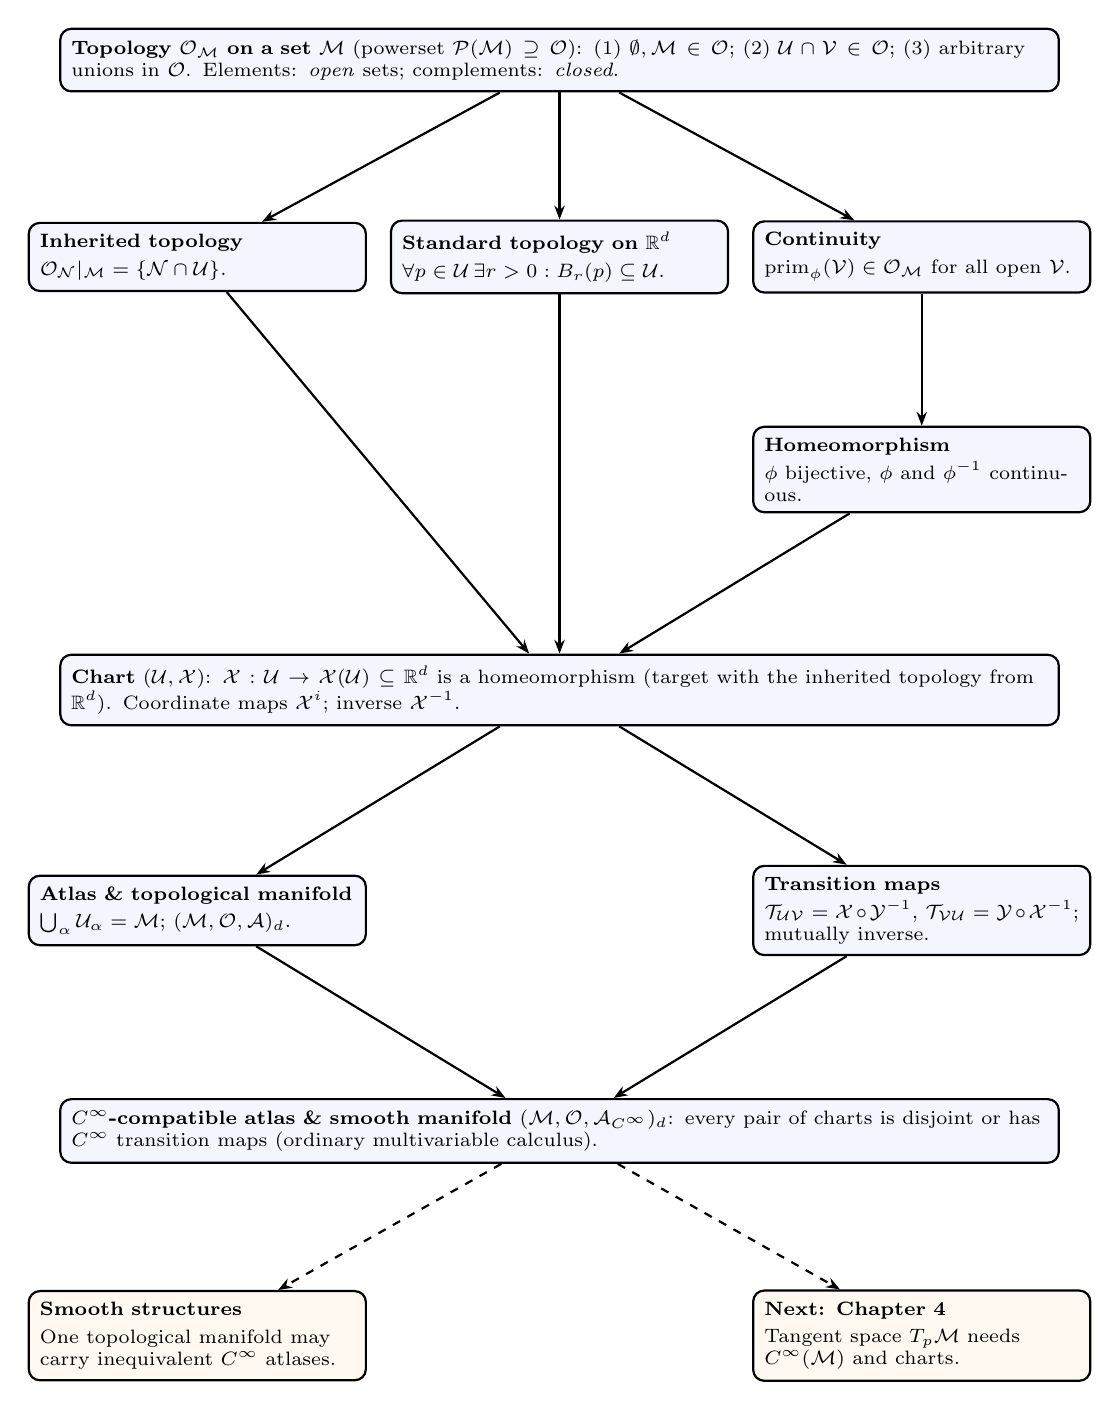
\begin{tikzpicture}[
  box/.style={draw, thick, rounded corners, fill=blue!4, align=left,
              text width=4.0cm, font=\scriptsize, inner sep=4pt},
  bigbox/.style={box, text width=12.4cm},
  aside/.style={box, text width=4.0cm, fill=orange!5},
  ->, >={Stealth[length=5pt]}, thick
]

\node[bigbox] (top) at (4.6,0) {%
  \textbf{Topology $\mathcal O_{\mathcal M}$ on a set $\mathcal M$} (powerset $\mathcal P(\mathcal M)\supseteq\mathcal O$):
  (1) $\emptyset,\mathcal M\in\mathcal O$; (2) $\mathcal U\cap\mathcal V\in\mathcal O$;
  (3) arbitrary unions in $\mathcal O$. Elements: \emph{open} sets; complements: \emph{closed}.
};

\node[box] (inh) at (0,-2.5) {%
  \textbf{Inherited topology}\\[2pt]
  $\mathcal O_{\mathcal N}|_{\mathcal M}=\{\mathcal N\cap\mathcal U\}$.
};
\node[box] (std) at (4.6,-2.5) {%
  \textbf{Standard topology on $\mathbb R^d$}\\[2pt]
  $\forall p\in\mathcal U\,\exists r>0: B_r(p)\subseteq\mathcal U$.
};
\node[box] (cont) at (9.2,-2.5) {%
  \textbf{Continuity}\\[2pt]
  $\mathrm{prim}_\phi(\mathcal V)\in\mathcal O_{\mathcal M}$ for all open $\mathcal V$.
};

\node[box] (homeo) at (9.2,-5.2) {%
  \textbf{Homeomorphism}\\[2pt]
  $\phi$ bijective, $\phi$ and $\phi^{-1}$ continuous.
};

\node[bigbox] (chart) at (4.6,-8.0) {%
  \textbf{Chart} $(\mathcal U,\mathcal X)$: $\mathcal X:\mathcal U\to\mathcal X(\mathcal U)\subseteq\mathbb R^d$ is a homeomorphism
  (target with the inherited topology from $\mathbb R^d$). Coordinate maps $\mathcal X^i$; inverse $\mathcal X^{-1}$.
};

\node[box] (atlas) at (0,-10.8) {%
  \textbf{Atlas \& topological manifold}\\[2pt]
  $\bigcup_\alpha\mathcal U_\alpha=\mathcal M$; $(\mathcal M,\mathcal O,\mathcal A)_d$.
};
\node[box] (trans) at (9.2,-10.8) {%
  \textbf{Transition maps}\\[2pt]
  $\mathcal T_{\mathcal U\mathcal V}=\mathcal X\circ\mathcal Y^{-1}$, $\mathcal T_{\mathcal V\mathcal U}=\mathcal Y\circ\mathcal X^{-1}$; mutually inverse.
};

\node[bigbox] (smooth) at (4.6,-13.6) {%
  \textbf{$C^\infty$-compatible atlas \& smooth manifold} $(\mathcal M,\mathcal O,\mathcal A_{C^\infty})_d$:
  every pair of charts is disjoint or has $C^\infty$ transition maps (ordinary multivariable calculus).
};

\node[aside] (smstr) at (0,-16.2) {%
  \textbf{Smooth structures}\\[2pt]
  One topological manifold may carry inequivalent $C^\infty$ atlases.
};
\node[aside] (next) at (9.2,-16.2) {%
  \textbf{Next: Chapter 4}\\[2pt]
  Tangent space $T_p\mathcal M$ needs $C^\infty(\mathcal M)$ and charts.
};

\draw (top) -- (inh);
\draw (top) -- (std);
\draw (top) -- (cont);
\draw (cont) -- (homeo);
\draw (inh) -- (chart);
\draw (std) -- (chart);
\draw (homeo) -- (chart);
\draw (chart) -- (atlas);
\draw (chart) -- (trans);
\draw (atlas) -- (smooth);
\draw (trans) -- (smooth);
\draw[dashed] (smooth) -- (smstr);
\draw[dashed] (smooth) -- (next);

\end{tikzpicture}%
}
\end{center}

\end{document}
